\section{Zusammenfassung und Ausblick} % (fold)
\label{sec:Zusammenfassung und Ausblick}

\subsection{Technologien und Forschung} % (fold)
\label{sub:Technologien}

Wie in den nächsten Abschnitten ersichtlich werden wird, ist die Entwicklung im Bereich Cloud und Edge Robotics sehr aktiv. Es ist daher einsehbar, dass in diesem Bereich ebenfalls viele Technologien folgen werden und aktuelle Entwicklungen ergänzt oder gar ersetzen werden. Im folgenden wird ein Ausblick auf aktuelle Entwicklungen geworfen die für die Anwendung im \acrlong{cttc} von Relevanz sind. Zum einen, werden im praktischen Kontext die geplanten Entwicklungen für das Zenoh Protokoll betrachtet die aber ebenfalls für generische Cloud und Edge Robotics Anwendungen wichtig sind. Zum anderen, wird ein Blick auf die Forschung beim Thema der Dataflow Programmierung gesetzt.

\subsubsection{Weiterentwicklungen in Zenoh} % (fold)
\label{ssub:Weiterentwicklungen in Zenoh}

Im Laufe dieser Arbeit wurde das Zenoh Protokoll vorgestellt und die Möglichkeiten zur Anwendung aufgezeigt. Zenoh wurde dabei gewählt, da es das Protokoll mit den passendsten Eigenschaften im Bezug auf die Kommunikation zwischen Robotern und dem Edge oder der Cloud ist. Trotz dessen, ist die Entwicklung des Protokolls noch am Anfang und enthält eine Roadmap \cite{Eclipsezenoh} mit einer Reihe von Features die für die weitere Nutzung im Cloud und Edge Bereich sehr nützlich sein können. Diese Konzepte kann man auch aus einer übergeordnete Perspektive sehen, da die meisten Ideen nicht auf Zenoh speziell beschränkt sind sondern auch im generellen Kontext der Roboterkommunikation eine Rolle spielen.\\
Unter den in der Roadmap für die Robotik interessant aufgeführten Features ist die Non Blocking Fault Tolerant Reliability, der Query Payload und der Connectivity Status. Diese könnten folgende Vorteile im für das Cloud und Edge Robotics bringen:

\begin{itemize}
  \item Non Blocking Fault Tolerant Reliability: In \ref{tab:qos} wurde die \code{RELIABILITY} Option vorgestellt. Mit diesem konnte man die Zuverlässigkeit einer Verbindung einstellen. In Falle eines Ausfalls des Routers und der dazugehörigen Änderung der Topologie, kann es zum Verlust von Paketen kommen. Da sich Zenoh aus Gründen der Skalierung nicht alle Verbindungen merkt, bringt die Non Blocking Fault Tolerant Reliability hier Abhilfe. Es tut dies, indem es ein Cache der bestehenden Verbindungen an anderen Orten im Netzwerk speichert. Dadurch können Verbindungen bei Ausfällen besser wiederhergestellt werden. Da Roboter als Publisher nicht sehr zuverlässig sind, würde dies im Cloud und Edge Robotics Bereich von Vorteil sein.
  \item Query Payload: Im Grundlagen Teil von Zenoh \ref{par:Zenoh Protokoll} wurden Selektoren und Key Expressions erläutert. Um in einer Query zusätzlich noch Daten in Form eines Payloads anzuhängen, wurde der Vorschlag des Query Payload erstellt. Der Payload wird dabei im \code{QueryBody} der Anfrage mitgeschickt. Zusätzlich werden Informationen wir das Encoding der Nachricht oder mit dem Flag \code{B} die Information ob Daten überhaupt mitgegeben wurden.
  \item Connectivity Status: Dieser ermöglicht es verschiedene Informationen aus den vorhandenen Verbindungen, in Zenoh \code{Session} genannt, zu entnehmen. Dieses Feature besteht dabei aus zwei Teilen. Zum einen soll man dadurch Informationen zu den bereits offenen Sessions bekommen. Zum anderen, soll man Benachrichtigungen über Ereignisse dieser Verbindungen bekommen können. Also Beispielsweise das Öffnen und Schließen von \code{Sessions}. Diese Schnittstellen können in der Anwendungslogik genutzt werden und Router erweiterte Möglichkeiten geben mit instabilen Verbindungen zurecht zu kommen.
\end{itemize}

% subsubsection Weiterentwicklungen in Zenoh (end)

\subsubsection{Dataflow Programmierung} % (fold)
\label{ssub:Dataflow Programmierung}

Das Konzept der Dataflow Programmierung basiert auf die Verarbeitung von Inputs in einem Flow von Daten. Im Kontext moderner Sprachen und grafischen Oberflächen wurde das Konzept im Jahre 2004 wieder untersucht \cite{johnstonAdvancesDataflowProgramming2004}. Dabei wurden verschiedenen Konzepte verglichen und die Frage gestellt, wie man Dataflow Programmierung in der Praxis anwenden könnte. In diesem Kontext wieder aufgegriffen wurde das Thema im Zuge der Cloud-to-Thing Forschung. Speziell, im V2X(Vehicle to X)\cite{baldoniZenohbasedDataflowFramework2021} Kontext. Ähnlich dem \acrlong{cttc}, geht es dabei um die Verbindung von IoT Geräten mit der Cloud. Bei V2X ist das ganze auf den Fahrzeugkontext bezogen.\\
Abstrakt gesehen, hat man bei der Dataflow Programmierung Knoten mit Operatoren. Knoten sind dabei Recheneinheiten. Operatoren können dabei die Input, Output oder Recheneigenschaft haben.

\begin{figure}
  \begin{center}
    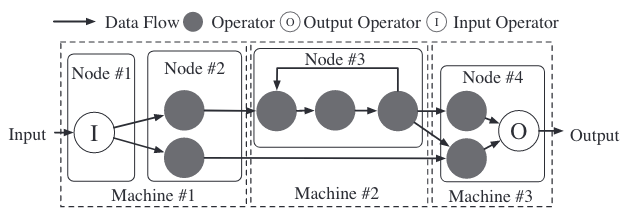
\includegraphics[width=0.95\textwidth]{figures/dataflow.png}
  \end{center}
  \caption{Dataflow Programmierung \cite{baldoniZenohbasedDataflowFramework2021}}
  \label{fig:dataflow}
\end{figure}

In Abbildung \ref{fig:dataflow} ist ein solch Abstraktes Beispiel dargestellt. Knoten 1 hat dabei ein Input Operator der den Datenflow auf zwei weitere Operatoren im Knoten 2 aufteilt. Die Knoten können sich dabei wie dargestellt auf mehreren Maschinen befinden. Knoten vier verbindet den Flow von zwei Operatoren wieder auf in ein Output.\\

Anwendungen können mit diesem Konzept unabhängig der Infrastruktur geplant werden und später mit einem spezielles Framework in die Realität umgesetzt werden. Ein Beispiel für solch ein Framework, ist die von Zenoh sich aktuell in der Entwicklung befindlichen Zenoh Flow Erweiterung. Diese nutzt die bereits behandelten Vorteile von Zenoh und konzentriert sich auf die Umsetzung von den Dataflow Konzepten. Die Umsetzung erfolgt relativ elegant mittels einer Infrastructure as Code Implementierung. Die Knoten und Operatoren werden dabei mit Hilfe einer YAML Syntax in einer deklarativen Art und Weise dargestellt. 

\begin{lstlisting}[caption={Beispiel einer YAML Datei für die Konfiguration von Zenoh Flow \cite{EclipseZenohFlowExamples2022}.}, label={lst:zenohflow}, captionpos=b]
flow: CountingPipeline
operators: []
sources:
  - id : Counter
    uri: file://./target/release/libcounter_source.so
    output:
      id: Counter
      type: usize
sinks:
  - id : PrintSink
    uri: file://./target/release/libgeneric_sink.so
    configuration:
      file: /tmp/generic-sink.txt
    input:
      id: Data
      type: usize

links:
- from:
    node : Counter
    output : Counter
  to:
    node : PrintSink
    input : Data
\end{lstlisting}

In \autoref{lst:zenohflow} wird dabei ein einfacher Zähler mit der Zenoh Flow Syntax beschrieben. Ein \code{Counter} Programm hat dabei einen Output, welcher den aktuellen Wert des Counters entspricht. Dazu gibt es noch ein \code{Sink} Programm welches den Wert als Input annimmt und ausgibt. Die Verbindung beider Objekte wird mittels \code{links} beschrieben.\\
Wie man hier klar erkennen kann, hat der Ansatz mit Hilfe von Infrastructure as Code den Vorteil die Konfiguration wiederverwendbar zu machen. Inspiration gibt es dabei an vielen Cloud Projekten wie Kubernetes oder Terraform die ebenfalls Infrastructure as Code für wiederverwendbare Beschreibungen von Architekturen nutzen.\\

Wie man sich vorstellen kann, eröffnet die Dataflow Programmierung eine noch Einfache Möglichkeit um Systeme wie in im Cloud und Edge Robotics Bereich zu verbinden. Ein Interessanter Use Case wäre die Auslagerung der Auswertung von Sensordaten in die Edge Schicht und die Verwendung der Berechnungsergebnisse wieder im Roboter. Der Roboter und die Edge Instanz wären dabei die beiden Involvierten Knoten. Ein Bewegungssensor im Roboter würde als Informationsquelle dienen, der an ein Output Operator angeschlossen ist. Die Informationen werden dabei zu beliebig vielen Berechnungsoperatoren im Edge geschickt. Nach der Berechnung kommen diese wieder in ein Input Operator am Roboter an und können zur Navigation verwendet werden.\\
Wie man also sehen kann, wendet Zenoh Flow das Konzept der Dataflow Programmierung an um die darunterliegende Infrastruktur soweit wie Möglich zu abstrahieren. Knoten und Operatoren durch \code{sources} und \code{sinks} mit den jeweiligen \code{input} und \code{output} Optionen. Vielversprechend ist auch die Abstraktion der Verbindungen. Diese werden in den \code{links} beschrieben und erstellen ein Zenoh Netzwerk. Die ganzen in dieser Arbeit beschriebenen Details müssen vom Entwickler nicht beachtet werden.

% subsubsection Dataflow Programmierung (end)

% subsection Technologien (end)

\subsection{Fazit} % (fold)
\label{sub:Fazit}

Wie in dieser Arbeit vorgestellt, ist das Thema Cloud und Edge Robotics sehr relevant. Dies lässt sich an verschiedenen Punkten erkennen. Zum einen, gibt es in diesem Bereich ein relativ Schnelllebiges Entwicklungsumfeld. Federführend ist dabei die Eclipse Foundation die hier mehrere Projekte unterstützt. Wie bereits erwähnt, entwickeln sich diese Projekt relativ schnell. Ein gutes Beispiel ist Fog05 ~\cite{EclipseFog052022}. Dieses war als als Ende zu Ende Lösung zum Provisionieren von Netzwerk, Speicher und Rechen Ressourcen in dezentralisierten Infrastrukturen gedacht\cite{corsaroFogO5UnifyingComputing2018}. Fog05 wurde ebenfalls unter der Eclipse Foundation entwickelt und wurde in relativ aktuellen Wissenschaftlichen Veröffentlichungen erwähnt. Trotz dessen, wurde die Entwicklung zu Gunsten des ebenfalls von Eclipse betreuten Zenoh Projektes ruhen gelassen. Projekte rund um Zenoh, wie die bereits erwähnte Zenoh Flow Erweiterung erfreuen sich immer größer werdenden Interesses. Zu sehen, an der aktiven in Entwicklung der Projekte auf dem Code Versionsverwaltungsdienst GitHub. In den dort entwickelten Projekten lässt sich ein positiver Trend in der Entwicklung von Cloud und Edge Robotik Projekten erkennen: Die wichtigsten Entwicklungen in diesem Bereich sind Open Source. Sowohl ROS2 als auch Zenoh und die weiteren in dieser Arbeit vorgestellten Technologien sind frei zur Nutzung verfügbar. Das ist ein wichtiger Faktor um in Zukunft den Bereich schneller wachsen zu lassen.\\

Neben der schnellen Entwicklung im praktischen Bereich, ist auch das Forschungsumfeld sehr aktiv. Im Bereich der Robotik, hat man mit ROS2 eine gute Grundlage gesetzt auf denen weitere Forschungen aufbauen können. Ein Vorteil aus den bereits bestehenden Grundladen, ist die Möglichkeit sich mit Themen zu beschäftigen, die sich mehr auf Nischen konzentrieren. Ein gutes Beispiel ist hier der Forschungsbereich rund um Robotik Systeme. Hier geht es immer mehr in Richtung spezielle Themen wie der Industriellen Anwendung oder dem autonomen Fahren. Dies steht im Gegensatz zu Forschungsergebnisse im Bereich des Edge Computings. Hier basieren viele Paper auf teilweise schon stillgelegte Konzepte wie das bereits erwähnte Fog05.\\

Trotz der positiven Signale im Entwicklungs und Forschungsbereich, ist die Perspektive für die Praxis aktuell noch nicht so klar. Wie in den vorherigen Abschnitten beschrieben, besteht noch kein klares Standard auf das man sich beruhen könnte. Trotz dessen, macht unter anderem die Eclipse Foundation im Edge und Cloud Bereich eine gute Arbeit, in dem es durch Kooperationen, Konferenzen und Projekte versucht Unternehmen auf Standard Technologien zu vereinen. Für die Industrie bedeutet es, dass es aktuell schwer ist sich auf eine bestimmte Technologie festzulegen. Viel mehr, ist es aktuell sinnvoller mit Proof of Concepts aktuelle Technologien zu testen und an der Entwicklung von neuen Möglichkeiten aktiv teilzuhaben.

% subsection Fazit (end)
